\section{Engine}
\label{verwendung_engine}
Wenn sie die FM3D-Engine in Kombination mit dem FM3D-Designer verwenden, so wird Ihnen bei der Projekterstellung ein funktionsfähiges VisualStudio C++ Projekt generiert, welches in der VisualStudio-Solution \textit{GameProject.sln} zu finden ist.
Es wird ihnen geraten, nichts an dem generierten Code zu ändern.
In der Datei \textit{"'presets.h"`} werden die Entity-Presets generiert, welche Sie im Designer erstellen können.
Sie können dem Projekt auch neue Dateien hinzufügen und unabhängig vom generierten Code programmieren. Weitere Dateien, welche ursprünglich nicht zu dem generierten Projekt gehört haben sollten keinen Einfluss auf die Funktionalität des generierten Codes haben.
Das Spiel an sich steht in der Main.cpp Datei, welche im Projekt bereits vorhanden ist.

\subsection{Voreinstellungen}
Zunächst müssen sie die Bibliotheken der FM3D-Engine, OpenGL, FreeImage, FreeType und Assimp in das Projekt einbinden. Falls Sie die Engine in Kombination mit dem FM3D-Designer verwenden, so werden die Verzeichnisse automatisch eingebunden. Falls nicht, so müssen Sie die Verzeichnisse manuell einbinden. Fügen Sie die Verzeichnisse in die zugehörige Option hinzu. Das ganze sollte so in ihren Einstellungen aussehen:
$$Configuration Properties->C/C++->Additional Include Directories$$\cref{includeinc}
$$Configuration Properties->Linker->Additional Include Directories$$
\cref{liblib}

\begin{figure}
	\begin{center}
		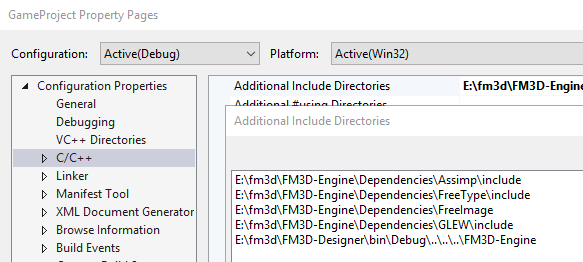
\includegraphics[width=\textwidth]{04verwendung/Engine/include.png}
		\caption{Include Verzeichnisse}\label{includeinc}
	\end{center}
\end{figure}

\begin{figure}
	\begin{center}
		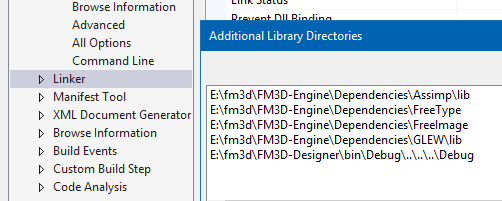
\includegraphics[width=\textwidth]{04verwendung/Engine/lib.png}
		\caption{Lib-Verzeichnisse}\label{liblib}
	\end{center}
\end{figure}

\subsection{Kamera}
Die Kamera ist in dem Generierten Projekt bereits vorhanden. Ihnen wird empfohlen die Werte der Position, Rotation und Zoom der Kamera im Bereich der \textit{Game-Logic} zu verändern. Auch dieser Bereich ist eindeutig mit Kommentaren kenntlich gemacht.

\subsection{Entities}
Erstellen Sie zunächst die Entities an der eindeutig kommentierten Stelle \textit{"'Create Entities here"`}. Dies geschieht mit dem folgenden Syntax:
%Beispiel
Wenn ein Entity das Komponent \textit{RenderableComponent} besitzt, so kann es in dem eindeutig kommentierten Abschnitt "'Submit objects here to renderer"` dem Renderer übergeben werden.
%Beispiel
Bevor Sie den Entities die Modelle zuweisen, vergessen Sie nicht die Modelle in die Projektmappe von VisualStudio zu laden.

\subsection{Inputsystem}
\label{inputsystemver}
Hierfür wird die Klasse \textit{Inputsystem} verwendet. Möchte man nun Tasten abfrage, so muss man zunächst auf die rekursive Instanz der Klasse zugreifen. 
$$FM3D::Inputsystem::GetInstance()->$$
Nun kann eine Methode aus dieser Klasse verwendet werden.
Möchten Sie nun abfragen, ob eine Taste der Tastatur gedrückt wurde, verwenden Sie die Methode
$$FM3D::Inputsystem::GetInstance()->CheckKey(int  keyid);$$
Der Integer-Wert \textit{keyid} bildet den ASCII-Code der zu abfragenden Taste ab. Die Methode gibt einen booleschen Wert zurück. Die Methode $$CheckMouse(int  keyid)$$ dient dem selben Zweck, nur wird hierbei der Status der Maus abgefragt.
Die Methode $$GetLastposClick(int keyID)$$
gibt einen zweidimensionalen Vektor vom Typ Float zurück, welcher die Position vom letzten Klick der Maus mit einer bestimmten Maustaste beschreibt. \textit{keyID} stellt die zu klickende Taste dar. 
$$GetLastposInst()$$
Die obenstehende Methode gibt Daten in Form eines zweidimensionalen Vektors mit der aktuellen Position der Maus zurück.

Alle Tasten der Tastatur und Maus können über Makros angesprochen werden. Auch können Sie die ASCII-Codes der einzelnen Tasten verwenden. Die Makros, welche die Tasten der Tastatur beschreiben starten mit \textit{"`KEY\_"'}. Die Makros, die für die Maus verwendet werden starten mit \textit{"`MAUS\_"'}.
